\scanpage{126}
\mspage{117}
% archive sheet number: 126

\uline{Corollaire 2} (Pour mémoire) Moyennant Hyp, \inserted{si $\Phi$ \unsure{irredondante|irredondant}} on a
\[
\begin{aligned}
\unsure{\mathrm{supp}^{\circ}|\mathrm{Supp}^{\circ}}(\Phi)&=\inserted{\mathrm{Omb}^{\circ}(\Phi)=}\mathrm{Omb}^{\circ}(\Phi_1)\cup\deleted{\unsure{\partial_0\cup\Delta_{\mathrm{is}}|\delta_0\cup\Delta_{\mathrm{is}}}}\Phi_0\\
&\deleted{{}=\bigcup_{\unsure{1\leq i\leq n}}\mathrm{Omb}^{\circ}(X_i)\cup\partial_0\cup\Delta_{\mathrm{is}}}
\end{aligned}
\]
(réunions disjointes).

\uline{Corollaire 3} Considérons la figure $\unsure{\Phi^{\prime *}|\Phi^{!*}}$ \deleted{formée}\inserted{définie} par

\deleted{1°) des \deleted{segments}\inserted{intervalles} interstitiels de $\Delta$ \unsure{qui ne sont} pas dans $\Phi$ i.e. qui \unsure{ne sont pas} dans $\mathrm{Omb}(\Psi)$, et}
\[
\deleted{\Phi_0^{\prime *}=\unsure{\delta|\partial}\Delta\setminus\Phi_0=\partial'_0}
\]

\[
\Phi_0^{\prime *}=\underbrace{\delta\Phi}_{\Delta}\setminus\Phi_0=\Delta\setminus\Phi_0=\Delta_{\mathrm{lac}}\amalg\partial'_0
\]
\margin{Rappel\newline
$\Delta=\Delta_{\mathrm{is}}\amalg\Delta_{\mathrm{int}}\amalg\partial\Psi$\newline
$\Phi_0=\Delta_{\mathrm{is}}\amalg\Delta_{\mathrm{red}}\amalg\partial_0$\newline
où $\Delta_{\mathrm{int}}=\Delta_{\mathrm{red}}\amalg\Delta_{\mathrm{lac}}$\newline
$\partial\Psi=\partial_0\amalg\partial'_0$}
où je pose
\[
\partial'_0\overset{\mathrm{def}}{=}\partial\Phi\setminus\partial_0\Phi=\unsure{\partial|\delta}\Psi\setminus\partial_0
\]
et
\[
\Phi_1^{\prime *}=\{\deleted{X\in\Phi_{\unsure{\Delta}}\cap\unsure{\mathcal{M}|M}_1\mid X\notin}\Phi_1\deleted{\unsure{\mathrm{Omb}(\Phi)|\mathrm{Omb}(\Phi_1)}}\}
\]
\[
\deleted{\unsure{=}}
\]
\figure{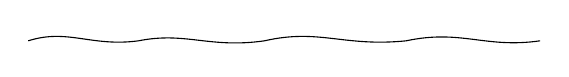
\begin{tikzpicture}\draw (0,0) .. controls (.5,.16) and (.8,-.08) .. (1.4,0) .. controls (2,.12) and (2.3,-.1) .. (3,0) .. controls (3.7,.16) and (4,-.08) .. (4.8,0) .. controls (5.5,.15) and (5.8,-.1) .. (6.5,0);\end{tikzpicture}}

Ça a l'air \unsure{fichtrement} compliqué comme présentation. Ne vaut il pas mieux dire ceci. Se donner une préfigure $\Phi$, c'est se donner

1°) $\Delta=\delta\Phi\in\mathrm{Drap}^{*}(\unsure{\mathcal{L}|L})$

2°) Une partie $\Phi_1\subset(\Phi_{\Delta})_1={}$ ens. des intervalles interstitiels de $\Delta$

3°) Une partie $\Phi_0\subset(\Phi_{\Delta})_0=\Delta$
